\section{Task 2: Reading Color Images}

Now it's time to look at some color images. First we have fruits.png:

\begin{figure}[H]
    \centering
    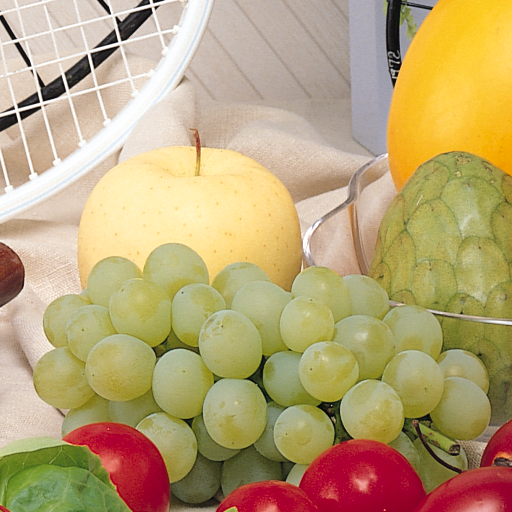
\includegraphics[scale=0.5]{fruits}
    \caption{Original fruits.png image}
\end{figure}

This image is a (mxnx3) image because it has three channels: Red, Green, and
Blue. For example, if we look at pixel (93,180) we get a value of (r,g,b),
again, each value represents Red, Green, and Blue intensities. If we separate
the image into its induvidual channels we get the following:

\begin{figure}[H]
    \centering
    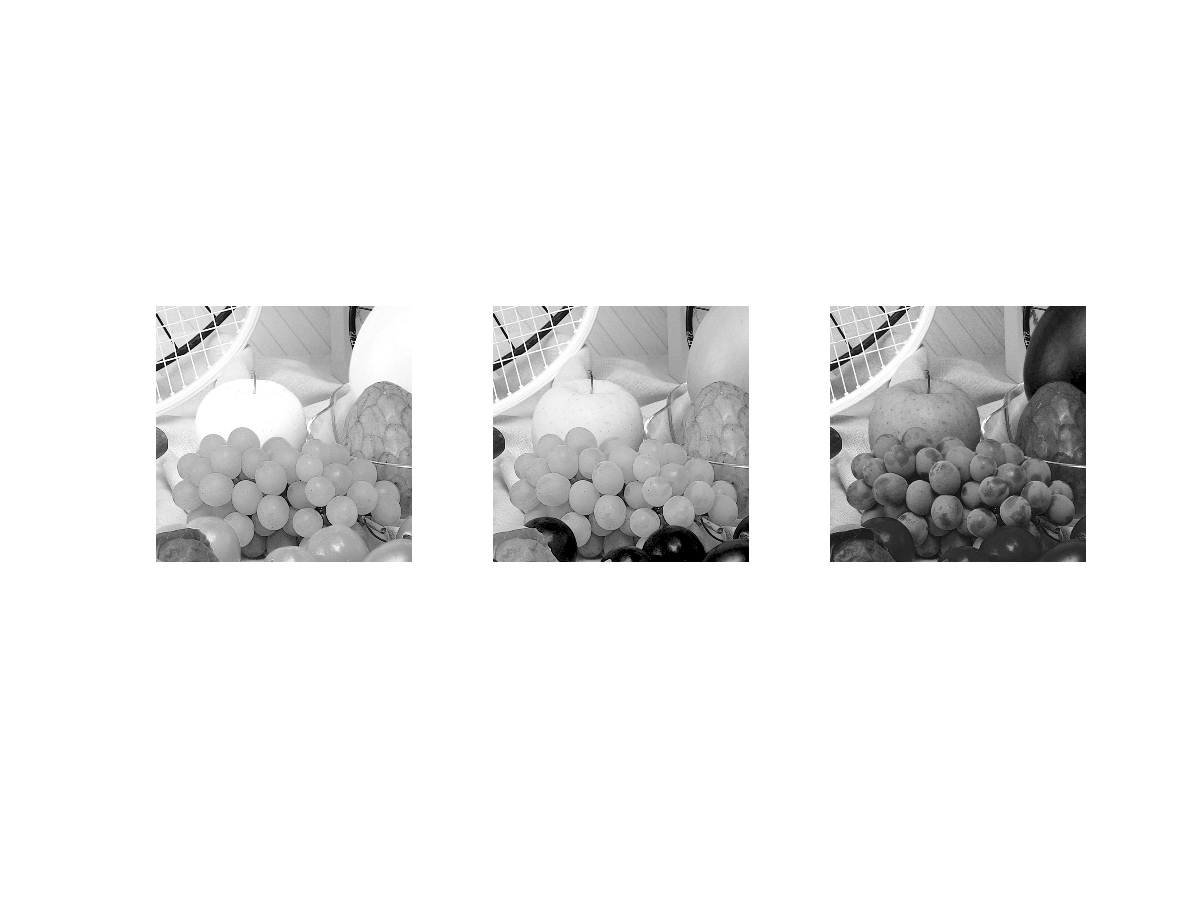
\includegraphics{threeChannels}
    \caption{Red, Green, and Blue channels of fruits.png}
\end{figure}

While the above images are in black and white, they represent the intensities of
their respective colors, so white in the "red" channel represents the red maximm
intensity of red. A white pixel in the original fruits image will be seen as
white in all three channels, as it is the max value for red, green, and blue.

Now I will convert fruits into an indexed image, I will index it with 16 and 256
colors. Indexed images can significantly reduce the memory taken up by an image
when there are few colors in said image. It does this by making an indexed table
of colors, the raw image data then becomes a single index value (instead of RGB)
which points to an RGB value in the table.

\begin{figure}[H]
    \centering
    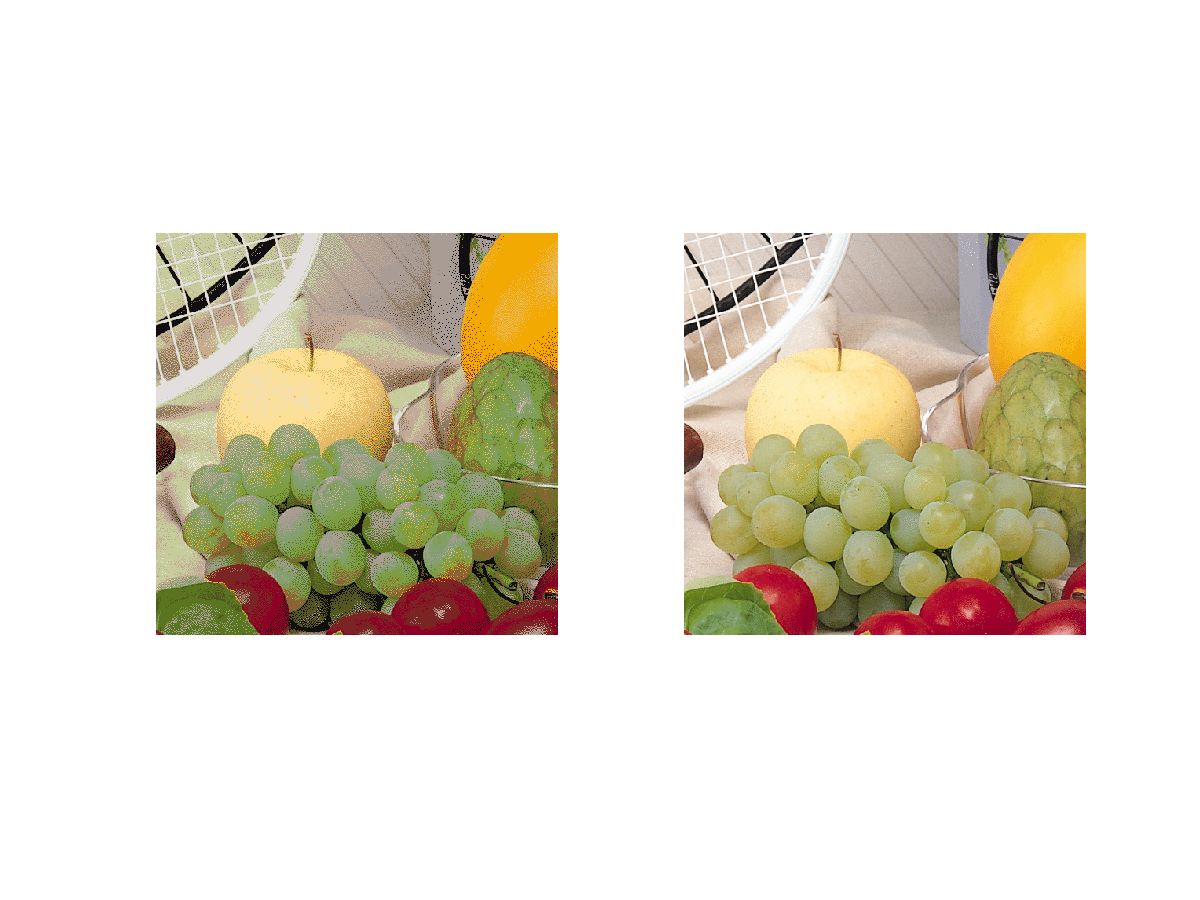
\includegraphics{indexed}
    \caption{256 and 16 indexed color image of fruits}
\end{figure}

If an image has many colors, the table can be made to be large to accomodate all
the colors, but then the indexed image does not save nearly as much memory,
which is the whole point of indexing! Alternatively the color table is kept
small, and much of the imformation in the image is lost. That is exactly what we
see in the above figure with 256 and 16 color indexing.
